\paragraph{QuizziPedia::Front-End::ModelViews::CreateQuestionnaireModelView}
	
	\label{QuizziPedia::Front-End::ModelViews::CreateQuestionnaireModelView}
	
	\begin{figure}[ht]
		\centering
		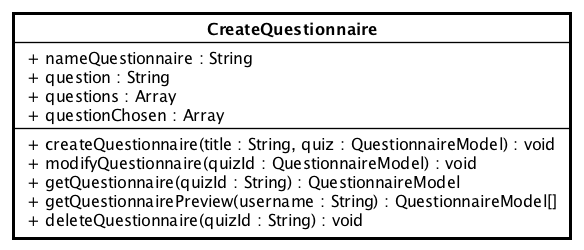
\includegraphics[scale=0.5,keepaspectratio]{UML/Classi/Front-End/QuizziPedia_Front-end_ModelView_CreateQuestionnaireModelView.png}
		\caption{QuizziPedia::Front-End::ModelViews::CreateQuestionnaireModelView}
	\end{figure} \FloatBarrier
	
	\begin{itemize}
		\item \textbf{Descrizione}: classe di tipo modelview la cui istanziazione è contenuta all'interno della variabile di ambiente \$scope di \textit{Angular.js\ped{G}}. All'interno di essa sono presenti le variabili e i metodi necessari per il \textit{Two-Way Data-Binding\ped{G}} tra la view \texttt{CreateQuestionnaireView} e il controller \texttt{CreateQuestionnaireController};
		\item \textbf{Utilizzo}: viene utilizzata per effettuare il \textit{Two-Way Data-Binding\ped{G}} tra la view \texttt{CreateQuestionnaireView} e il controller \texttt{CreateQuestionnaireController} rendendo disponibili variabili e metodi;
		\item \textbf{Relazioni con altre classi}: 
		\begin{itemize}
			\item \textit{OUT} \texttt{CreateQuestionnaireView}: view per la creazione del questionario; 
			\item \textit{OUT} \texttt{CreateQuestionnaireController}: questa classe permette di gestire la creazione di un questionario;
		\end{itemize}
		\item \textbf{Attributi}: 
		\begin{itemize}
			\item \texttt{+ nameQuestionnaire: String}: \\ Attributo che specifica il nome del questionario creato;
			\item \texttt{+ question: String} \\ Attributo che conterrà la stringa per la ricerca della domanda;
			\item \texttt{+ questions: Array} \\ Array contenente le domande trovate durante la ricerca;
			\item \texttt{+ questionsChosen: Array} \\ Array contenente le domande inserite nel questionario.
		\end{itemize}
		\item \textbf{Metodi}: 
		\begin{itemize}
			\item \texttt{+} \texttt{createQuestionnaire(title: String, quiz: QuestionnaireModel) : Void}: \\Metodo che permette di inserire un questionario nel database tramite richiesta al service; \\
			\textbf{Parametri}:
			\begin{itemize}
				\item \texttt{title: String} \\ Parametro che indica il nome del questionario;
				\item \texttt{quiz: QuestionnaireModel} \\ Parametro che racchiude tutti i dati di un questionario.
			\end{itemize}
			\item \texttt{+} \texttt{modifyQuestionnaire(quizId: QuestionnaireModel): void}: \\ Metodo che serve per modificare un questionario; \\
			\textbf{Parametri}:
			\begin{itemize}
				\item \texttt{quiz: QuestionnaireModel}: parametro che rappresenta l'oggetto questionario;
			\end{itemize}
			\item \texttt{+} \texttt{getQuestionnaire(quizId: String): QuestionnaireModel}: \\Metodo che serve per ottenere un questionario tramite l'id in modo da poterlo modificare; \\
			\textbf{Parametri}:
			\begin{itemize}
				\item \texttt{quizId: String}: parametro che rappresenta l'id del questionario da richiedere.
			\end{itemize}
			\item \texttt{+} \texttt{getQuestionnairePreview(username: String)}: \\ Metodo che serve per ottenere la lista di tutti i questionari di un utente; \\
			\textbf{Parametri}:
			\begin{itemize}
				\item \texttt{username: String}: parametro che indica l'utente del quale vogliamo caricare tutti i questionari.
			\end{itemize}
			\item \texttt{+} \texttt{deleteQuestionnaire(quizId: String): void}: \\Metodo che elimina un questionario.
			\textbf{Parametri}:
			\texttt{quizId: String}: identificativo del questionario da eliminare.
		\end{itemize}
	\end{itemize}
	
	